\documentclass{article}

\usepackage{geometry}
\geometry{margin=2cm}
\usepackage{graphicx}
\usepackage{hyperref}
\usepackage{amsfonts}

\hypersetup{colorlinks=true, linkcolor=blue, urlcolor=blue, citecolor=blue}
\urlstyle{same}
\begin{document}
	
	\author{Aayush Arya}
	\date{(Submitted: September 14, 2021)}
	\title{}
	
	\maketitle
	
	\hrule
	\begin{center}
		PHY382 Lab Report\\
		Practical: 3 \quad Registration No.: 11912610 \quad Section: G2903
	\end{center}
	\hrule
	
	\section*{Introduction to Fourier transforms}
	The concept of a Fourier {\it series} lets one expand a function $f(x)$ defined over a finite interval $[a,b]$ as a sum of infinite $e^{ikx}$ over a discrete spectrum of frequencies corresponding to values of $k$.\\
	
	 However, there's a technique for writing functions in terms of a continuous set of frequencies, without the requirement of assuming that the function needs to be periodic over a finite interval. In fact, one can apply the operation \textemdash called a {\it Fourier transform} \textemdash to functions defined over the entirety of $\mathbb{R}$ (or more generally, over $\mathbb{R}^n$ for vector-valued functions), with no periodicity. The only thing we require is that $\int_\mathbb{R} |f(x)|dx$ be finite. Note that this immediately means that an $f$ belonging to the Banach space $L^1_\mathbb{C}(\mathbb{R}^n)$ would automatically satisfy this requirement.
	
	\subsection*{From discrete to continuum}
	
	For a function $f(t)$ periodic over an interval $T$, its Fourier expansion is \begin{equation}
		f(t) = \sum_{r=-\infty}^{\infty}c_r e^{2\pi i rt/T}
	\end{equation}
	
	One could write $2\pi r/T = \omega_r$, where the discrete frequencies $\omega_r$ differ from each other by $\Delta\omega \equiv 2\pi/T$. The coefficients (amplitudes of the harmonics) were given by
	
	$$ c_r = \frac{1}{T}  \int_{-\infty}^{\infty} f(t) e^{-i\omega_r t} dt =
	 \frac{\Delta\omega}{2\pi}  \int_{-T/2}^{T/2} f(t) e^{-i\omega_r t} dt$$
	
	\begin{figure}[h!]
		\centering
		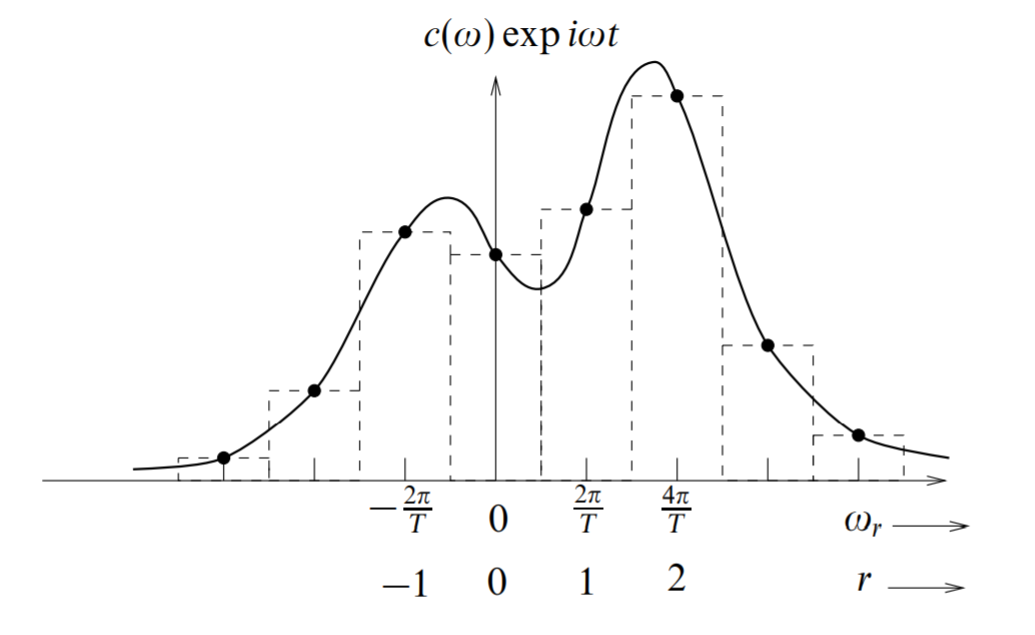
\includegraphics[width=0.4\textwidth]{integral_fig}
		\caption{The relation between discrete $c_r e^{i\omega_r t}$ and a continuous Fourier spectrum. The sum of the area of the rectangles (each corresponding a different $\omega_r$) of width $\Delta \omega = 2\pi/T$ in the limit $\Delta \omega \to 0$ converges to the area under the curve. Figure reprinted from reference \cite{riley+}.}
		
	\end{figure}
	
	If we allow our function to have a time period $T \to \infty$, that's equivalent to no apparent periodicity over the entirety of the real line $\mathbb{R}$. An arbitrarily large time period also corresponds to a vanishingly small frequency quantum $\Delta \omega$. In that limit, the discrete Fourier sum becomes an integral.
	
	Therefore, if we plug in the value of $c_r$ from the equation above into (1),
	
	$$  f(t) = \sum_{r=-\infty}^{\infty} \frac{\Delta\omega}{2\pi}\left(\int_{-\infty}^{\infty} f(u) e^{-i\omega_r u} du \right) e^{i\omega t}$$
	
	where we have changed the variables from $t$ to $u$ while substituting $c_r$ to avoid confusion, since the $e^{i\omega t}$ outside is not supposed to be part of the integral.
	
	
	This in the limit $T\to \infty$, $\Delta \omega \to 0$ becomes an integral
	
	$$ f(t) = \frac{1}{2\pi} \int_{-\infty}^{\infty} e^{i\omega t} d\omega \int_{-\infty}^{\infty} f(t)e^{-i\omega t} dt$$
	
	We note that the integral with respect to $dt$ is nothing but a form of the amplitude (or coefficient) $c_r$. We refer to this amplitude as $$\tilde{f}(\omega) = \frac{1}{\sqrt{2\pi}} \int_{-\infty}^{\infty} f(t)e^{-i\omega t} dt $$
	where the $1/\sqrt{2\pi}$ has been used for a symmetric defintion, such that
	$$ f(t) = \frac{1}{\sqrt{2\pi}} \int_{-\infty}^{\infty} \tilde{f}(\omega)e^{i\omega t} d\omega $$
	
	\section*{Importance \& Applications}
	
	Fourier transforms are of fundamental importance in quantum mechanics, where the state vectors (wavefunctions) are elements of the Hilbert space $L^2$ of square integrable functions. One special feature of $L^2_{\mathbb{C}}(\mathbb{R}^n)$ is that it is self-dual (this is not true for an arbitrary space). What this means is that the Fourier transform of a $\psi$ would map from and to the same vector space $L^2_{C}(\mathbb{R}^n) \to L^2_{C}(\mathbb{R}^n)$\cite{Lukas}. Therefore, $\psi(x)$ and $\tilde{\psi}(k)$ lie in the same vector space. \\
	
	But it's not only important for a mathematical formalism. They are important in different forms of spectroscopy, including Fourier Transform Infrared Spectroscopy (FT-IR), a form of mass spectroscopy (FT-ICR-MS) which require Fourier transforms for reconstructing signals into useful forms.
	
	Fourier transforms are essential for making crystal X-Ray Diffraction data interpretable pictorially, reconstructing signals in observational astronomy problems, etc.
	
	
	
	\section*{Learning Outcomes}
	
	I learnt how the notion of series expansion using discrete sums with the basis $\{e^{i\omega_r t} | r \in \mathbb{R} \}$ due to Fourier can be extended to an integral expansion (in the continuum limit of $\Delta \omega \to 0$). It's astonishing how this makes it applicable to functions without any inherent periodicity.
	
	\begin{thebibliography}{widestlabel}
		\bibitem{riley+} K. F. Riley, M. P. Hobson, S. J. Bence (2006). {\it Mathematical Methods for Physics and Engineering} ($3^{rd}$ Edition). Cambridge University Press.
		
		\bibitem{Lukas} [Lecture Notes] Lukas, Andre (2018). {\it Mathematical Methods}. Available: \url{http://www-thphys.physics.ox.ac.uk/people/AndreLukas/MathMeth/}
		
	\end{thebibliography}
\end{document}